\subsection*{Problema 08}

\textbf{Enunciado:} \\
Calcular la integral indefinida:
\begin{align*}
\int \dfrac{2x^2 + 3}{x^3 - 2x^2 + x} \, dx
\end{align*}

\textbf{Solución:} \\
Primero, factorizamos el denominador de la función racional:
\begin{align*}
x^3 - 2x^2 + x &= x(x^2 - 2x + 1) \\
&= x(x - 1)^2
\end{align*}

Planteamos la descomposición en fracciones parciales sugerida:
\begin{align*}
\dfrac{2x^2 + 3}{x(x - 1)^2} = \dfrac{A}{x} + \dfrac{B}{x - 1} + \dfrac{C}{(x - 1)^2}
\end{align*}

Multiplicamos toda la ecuación por el denominador común $x(x - 1)^2$:
\begin{align*}
2x^2 + 3 &= A(x - 1)^2 \\
&\quad + Bx(x - 1) + Cx
\end{align*}

Para hallar los valores de las constantes, evaluamos en valores convenientes de $x$:

Si $x = 0$:
\begin{align*}
2(0)^2 + 3 &= A(0 - 1)^2 + 0 + 0 \\
3 &= A(1) \implies A = 3
\end{align*}

Si $x = 1$:
\begin{align*}
2(1)^2 + 3 &= 0 + 0 + C(1) \\
5 &= C \implies C = 5
\end{align*}

Para hallar $B$, usamos $x = 2$ y el valor de $A = 3$, $C = 5$:
\begin{align*}
2(2)^2 + 3 &= 3(2 - 1)^2 \\
&\quad + B(2)(2 - 1) + 5(2) \\
11 &= 3(1) + 2B + 10 \\
11 &= 13 + 2B \implies 2B = -2 \\
B &= -1
\end{align*}

Sustituimos las constantes $A$, $B$ y $C$ en la integral:
\begin{align*}
\int &\left( \dfrac{3}{x} - \dfrac{1}{x - 1} + \dfrac{5}{(x - 1)^2} \right) dx
\end{align*}

integramos término a término:
\begin{align*}
&= 3\ln|x| - \ln|x - 1| \\
&\quad - \dfrac{5}{x - 1} + K
\end{align*}

Por lo tanto, la solución general es:
\begin{align*}
\int &\dfrac{2x^2 + 3}{x^3 - 2x^2 + x} \, dx \\
&= \ln\left|\dfrac{x^3}{x - 1}\right| - \dfrac{5}{x - 1} + K
\end{align*}

\begin{figure}[H]
	\centering
	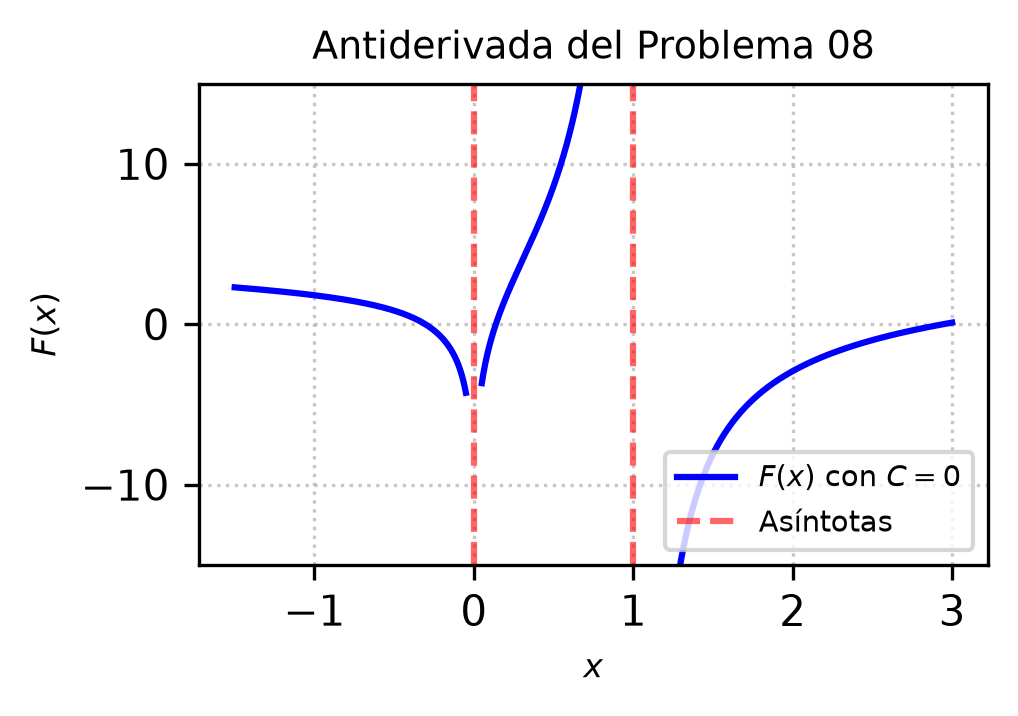
\includegraphics[width=\columnwidth]{semana_03/graficas/SEM03_P08_grafica.png}
	\caption{Representación gráfica de $f(x)$ y su antiderivada $F(x)$ evaluada para la constante de integración $C = 0$ (Problema 08).}
	\label{fig:problema08}
\end{figure}
